\subsection{Clustering}\label{sec:ts_clustering}
In our clustering analysis of time series we adopted two different approaches to the measure of similarity: shape-based similarity and structural similarity.

For the shape-based approach, we first subjected the time series to amplitude scaling and then measured the distances between records employing DTW as to minimize the impact of misaligned time series.
Since our time series were very short, we didn't deem it necessary to apply any approximation method to the original signal; we did, however impose constraints (Sakoe-Chiba Band with radius 0.1) on the warping in order to reduce computation time and avoid pathological warpings.

For the global structural approach, we extracted mean, standard deviation and Catch22 features from the raw signals (without amplitude scaling) and then computed Euclidean Distance on this new feature matrix (which was normalized using a Standard Scaler).

\subsubsection{Shape-based clustering}

\begin{figure}
    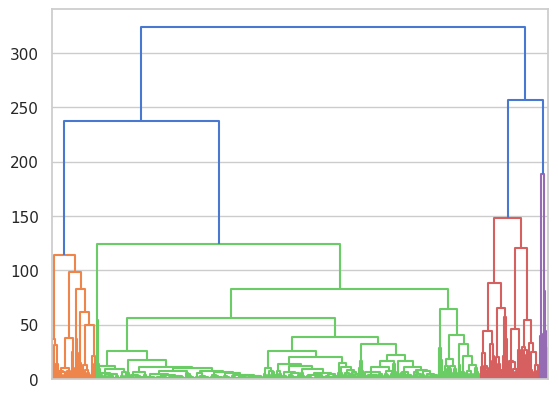
\includegraphics[width=\columnwidth]{../results/images/tsclust_hierarhical_dendrogram.png}
    \caption{Dendrogram for shape-based hierarhical clustering.}\label{fig:tsclust_dendrogram}
\end{figure}

\begin{figure}
    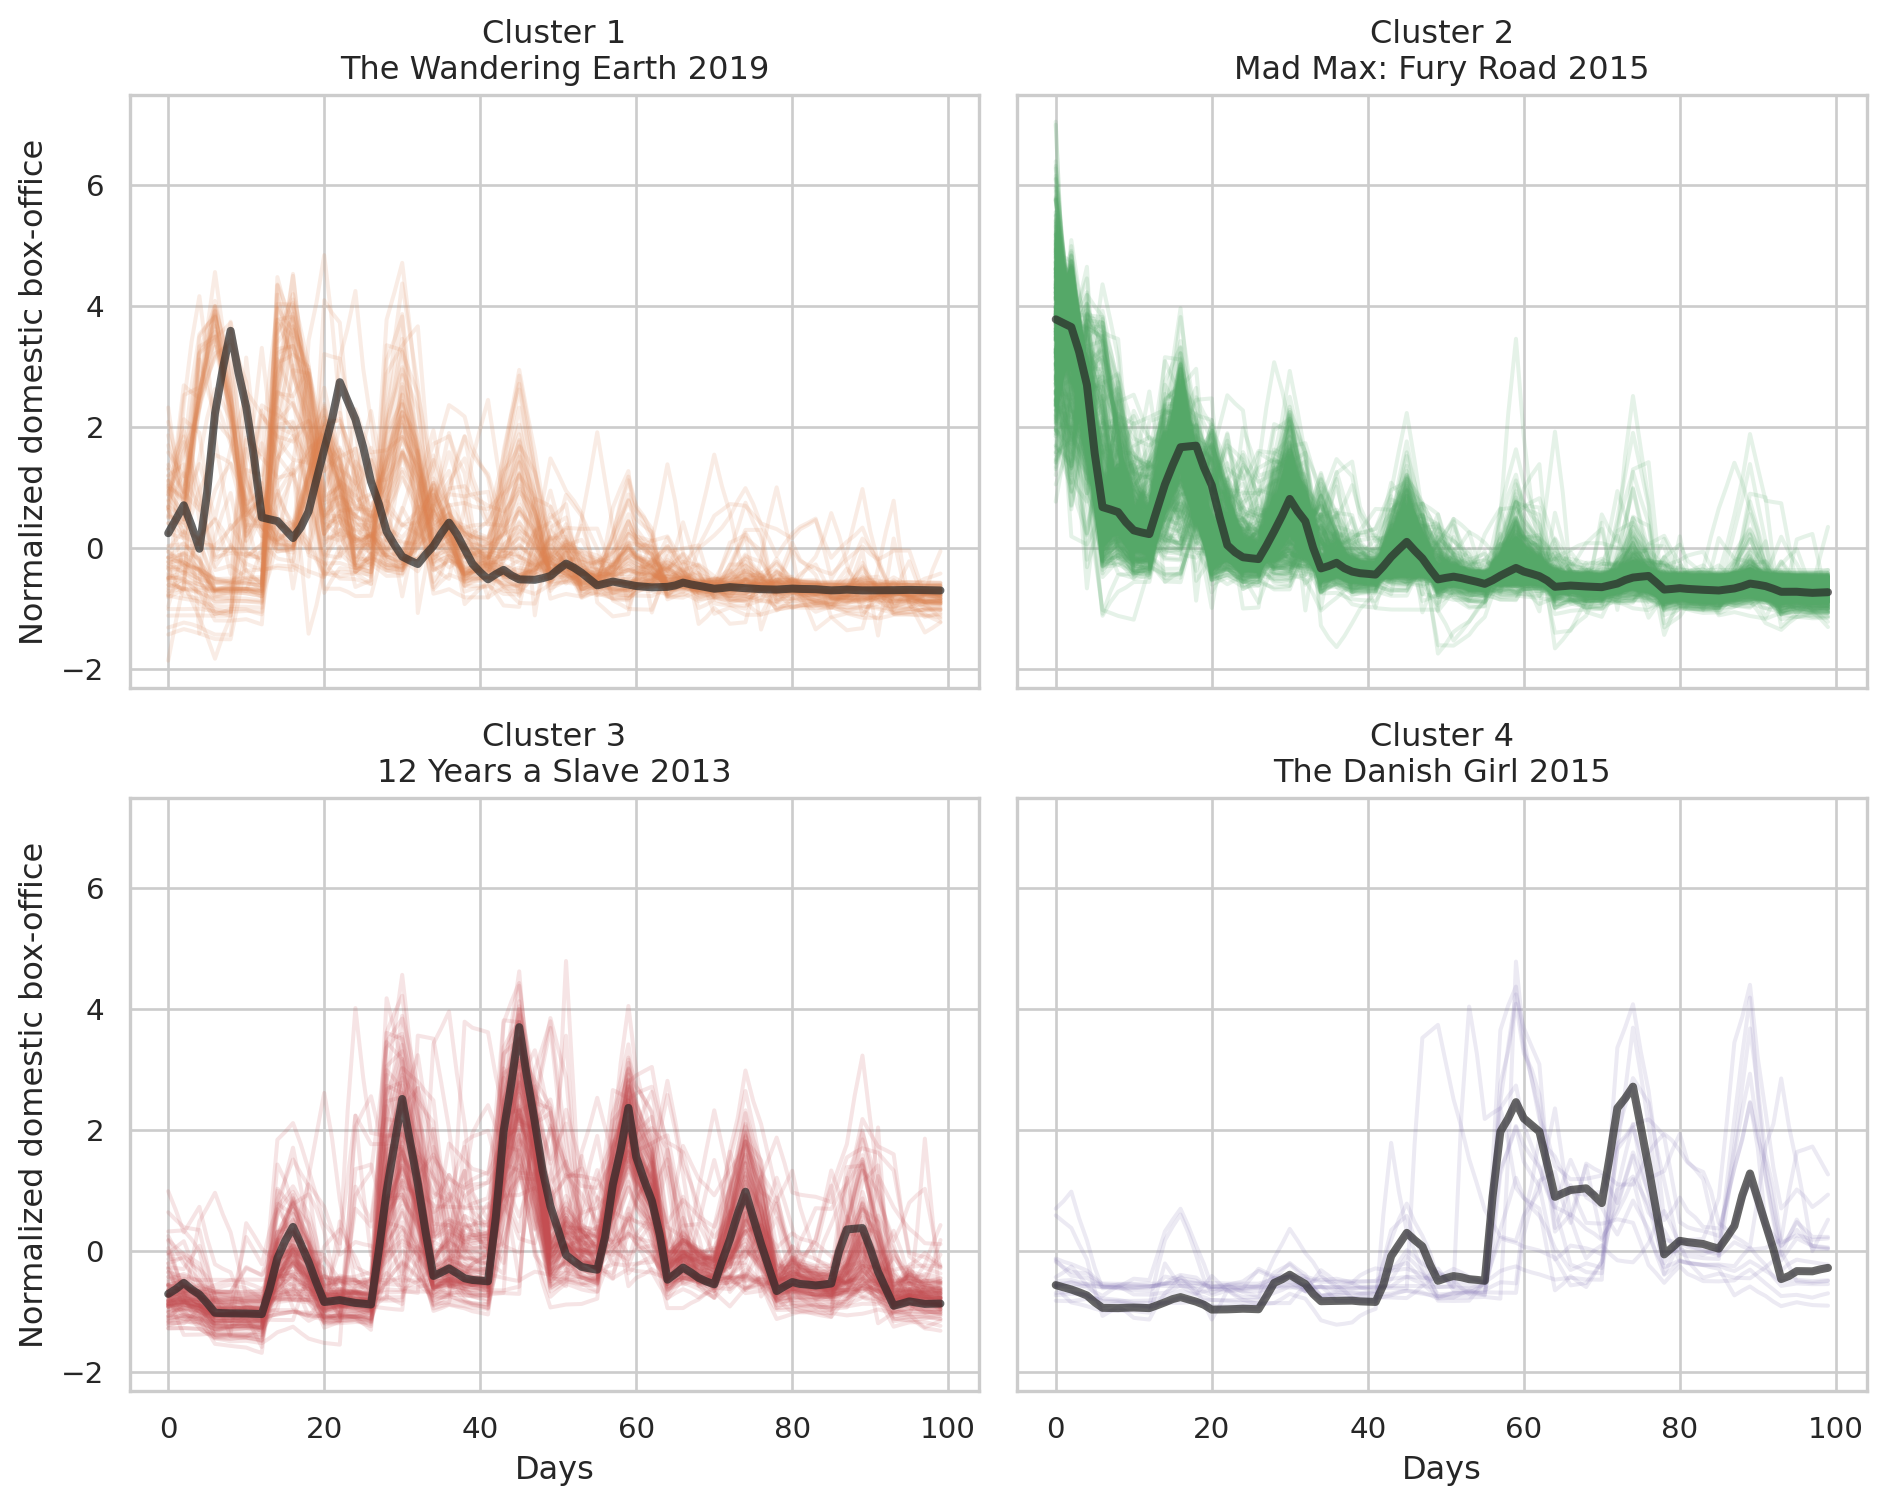
\includegraphics[width=\columnwidth]{../results/images/tsclust_hierarhical_series.png}
    \caption{Clusters obtained by hierarchical clustering and respective cluster medoids (in black).}\label{fig:tsclust_hierarchical_series}
\end{figure}

\begin{figure}
    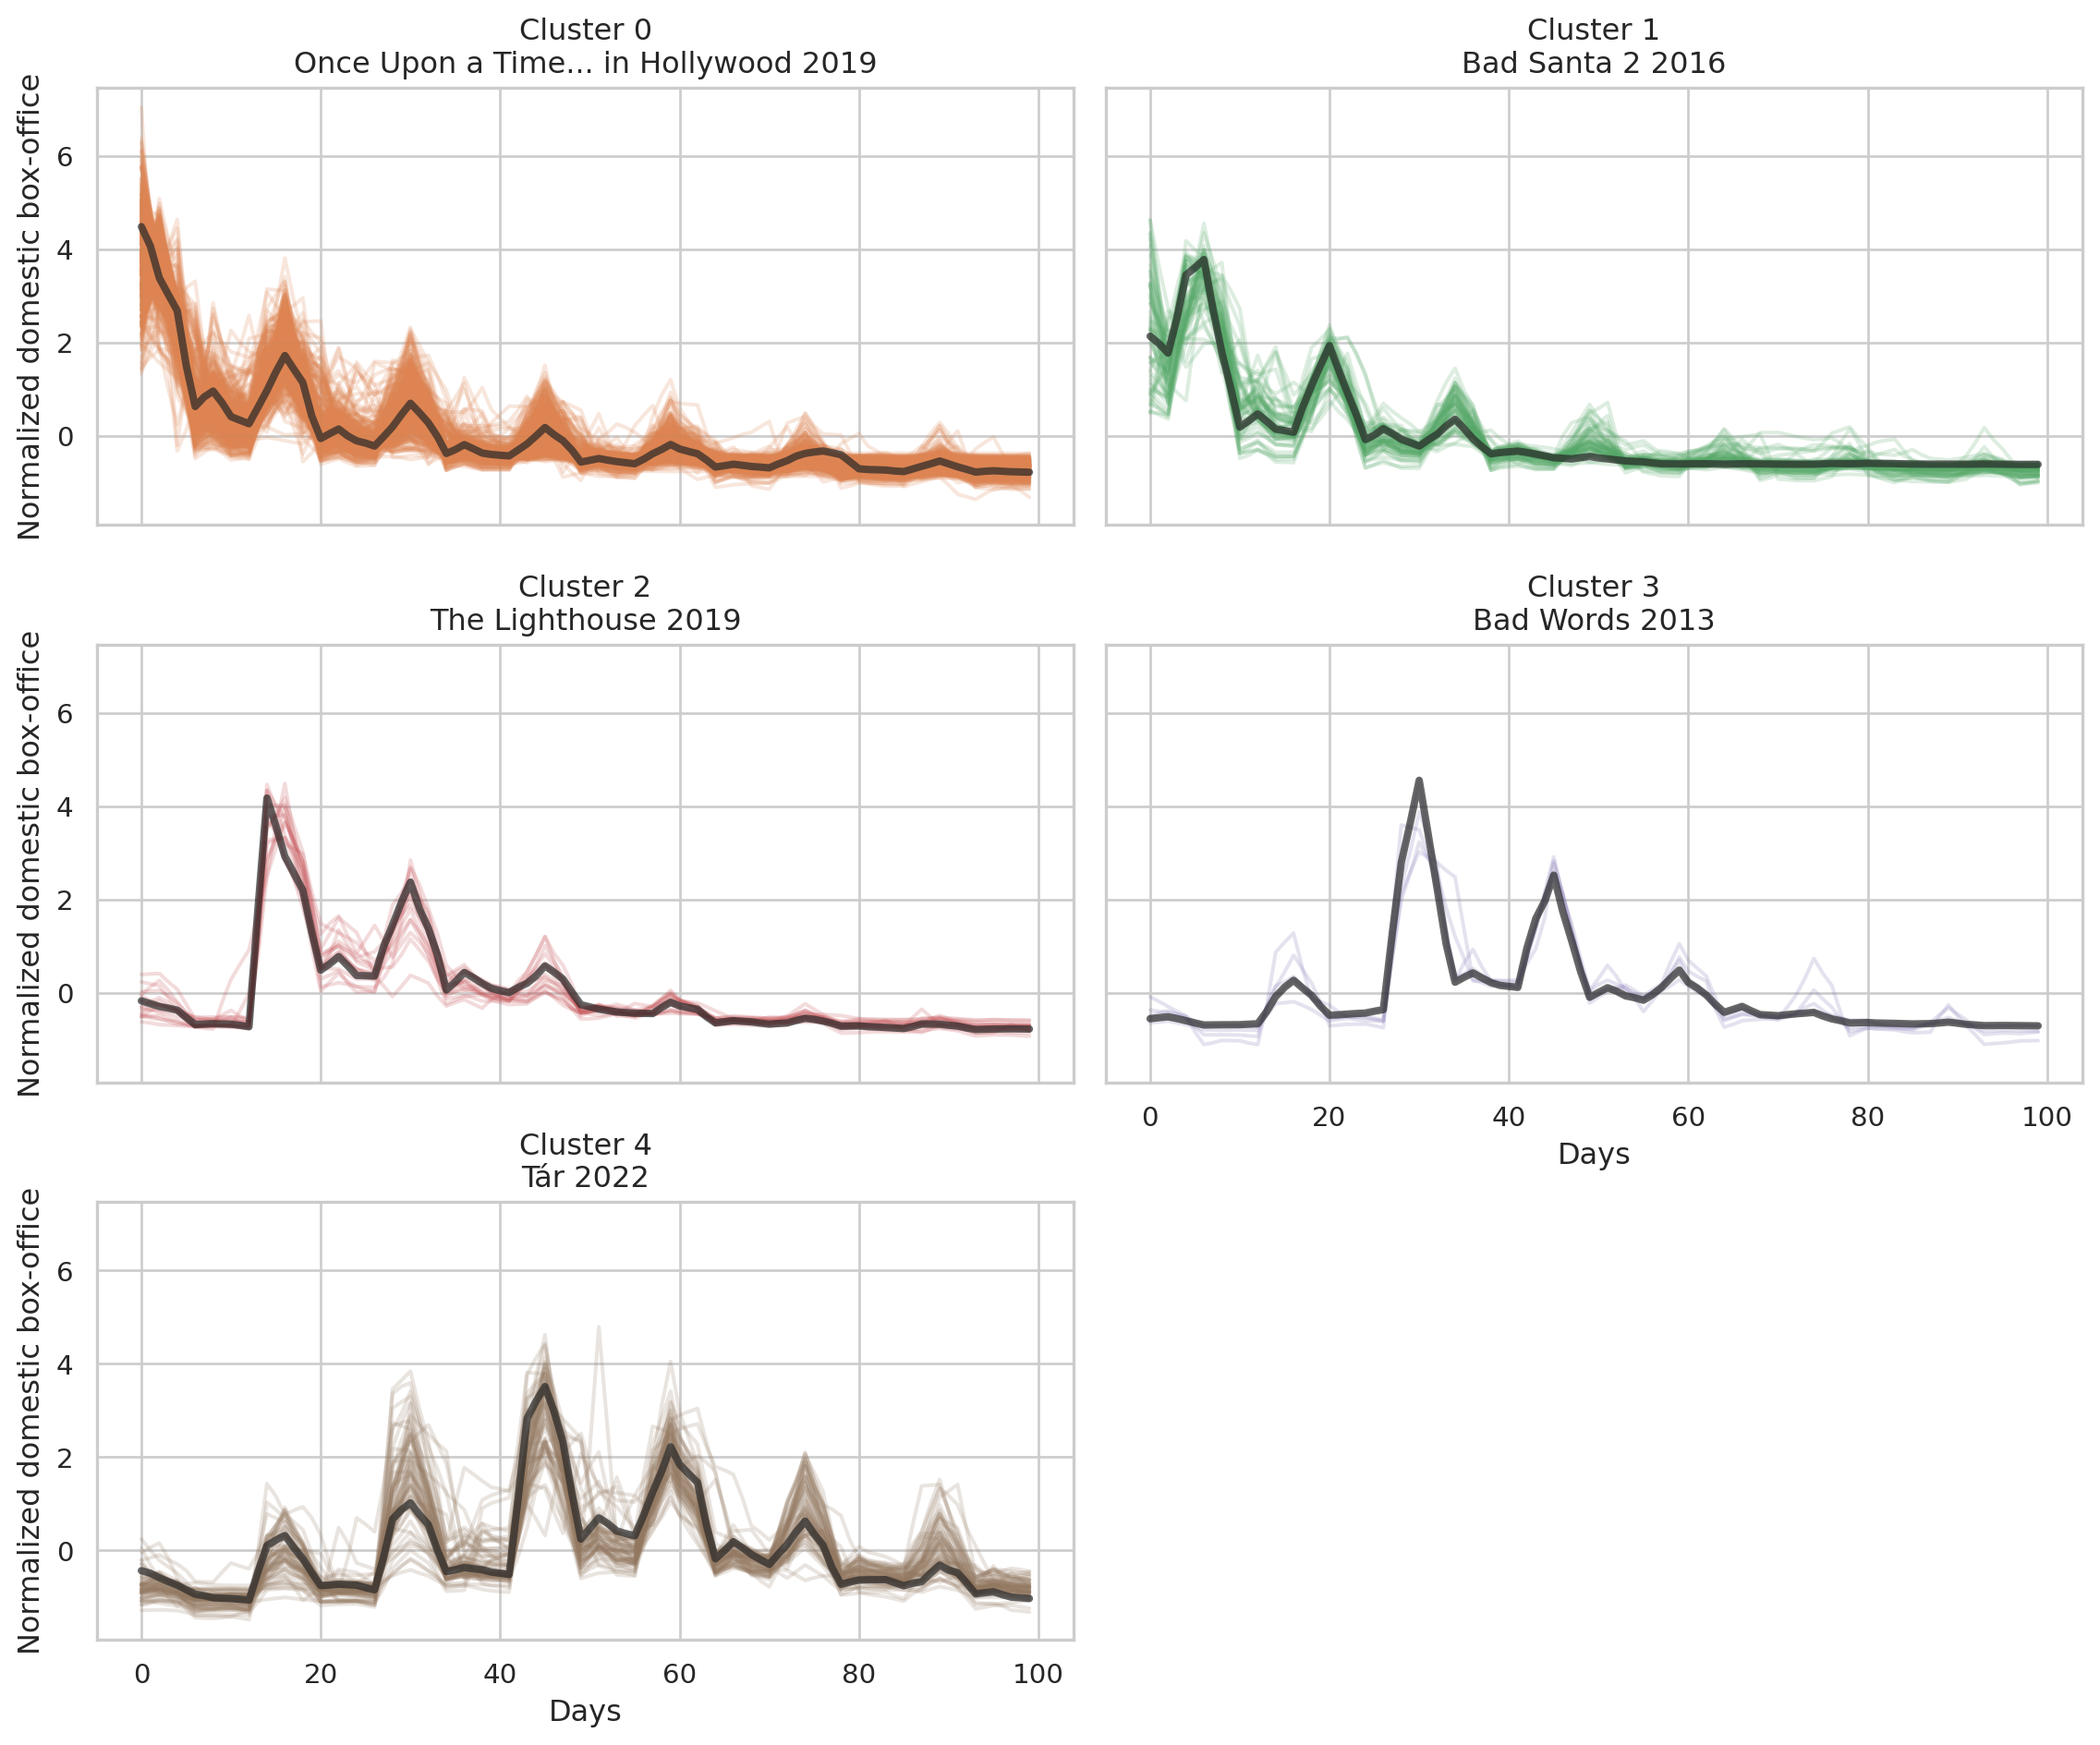
\includegraphics[width=\columnwidth]{../results/images/tsclust_density_series.png}
    \caption{Clusters obtained by density-based clustering and respective cluster medoids (in black).}\label{fig:tsclust_density_series}
\end{figure}

Since in our understanding phase we were able to recognize two distinct patterns, we first of all run K-Means with k=2 and obtained results very similar to those previously discussed. This clustering obtained a silhouette score of 0.85 and was able to identify 159 `late bloomers'.

We then experimented with different linkage criteria for hierarchical clustering, selecting in the end average linkage, which yielded the best dendrogram (Fig. \ref{fig:tsclust_dendrogram}).
After selecting an appropriate threshold, we obtained 4 clusters of very different sizes (C1: 75, C2: 658, C3: 101, C4:15). This clustering obtained a silhouette score of 0.77.

Signals for clustered time series and cluster medoids are visualized in Fig. \ref{fig:tsclust_hierarchical_series}: it can be easily seen that, while C2 and C3 can be identified respectively with instant hits and `late bloomers', the identity of movies from C1 and C4 is more confused.
Detailed analysis of silhouette scores revealed that many records from C4 and especially C1 have negative silhouette scores, suggesting that they were assigned to the wrong cluster.

We then run Principal Component Analysis on the dataset and visualized clusters on the two first components, which together explain more than 60\% of variance (Fig. \ref{fig:hier_pca}, cluster medoids are showed in black).

Inspecting the PCA Eigenvectors, we found out that the first component is mainly concerned with timestamps from the first week or so, which explains why records from C2 (and some records from C1) have positive values in this component, while the `late bloomers' from C3 have very negative values.
Also, observing the distribution of records from C1 along the first component, it is clear why more than half of them have a negative silhouette score, since they clearly should belong to C2.
In contrast, K-Means, clearly separates the two clusters along the first component.

\begin{figure*}[t]
    \centering
    \begin{subfigure}{0.45\textwidth}
        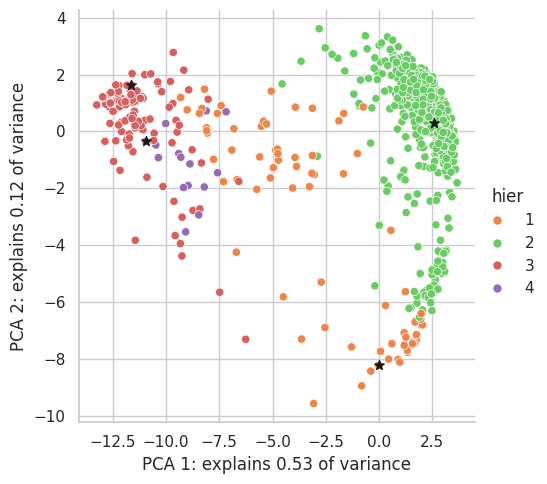
\includegraphics[width=\textwidth]{../results/images/tsclust_hier_pca.png}
        \caption{Hierachical clustering PCA.}\label{fig:hier_pca}
    \end{subfigure}
    \begin{subfigure}{0.45\textwidth}
        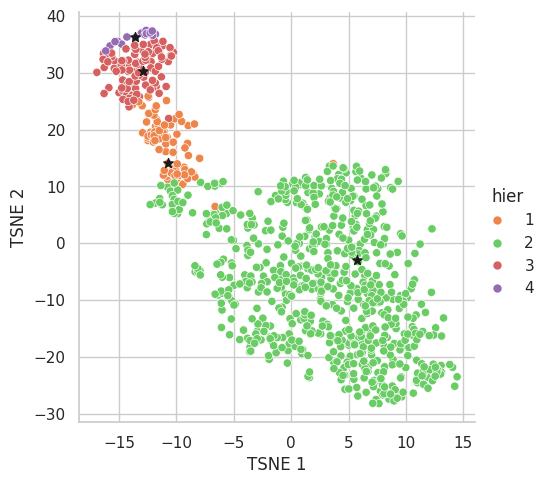
\includegraphics[width=\textwidth]{../results/images/tsclust_hier_tsne.png}
        \caption{Hierarchical clustering tSNE.}
    \end{subfigure}
    \begin{subfigure}{0.45\textwidth}
        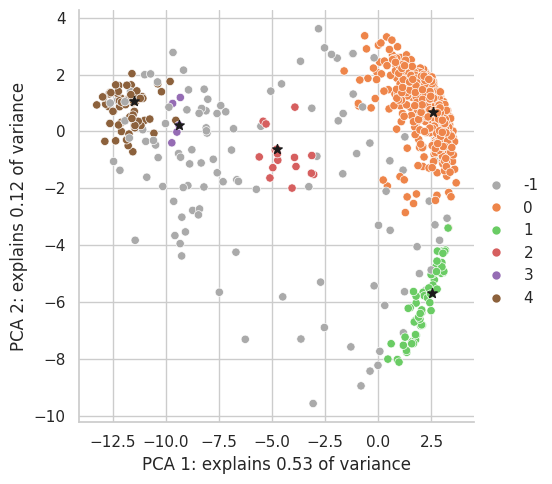
\includegraphics[width=\textwidth]{../results/images/tsclust_density_pca.png}
        \caption{DBSCAN clustering PCA.}\label{fig:density_pca}
    \end{subfigure}
    \begin{subfigure}{0.45\textwidth}
        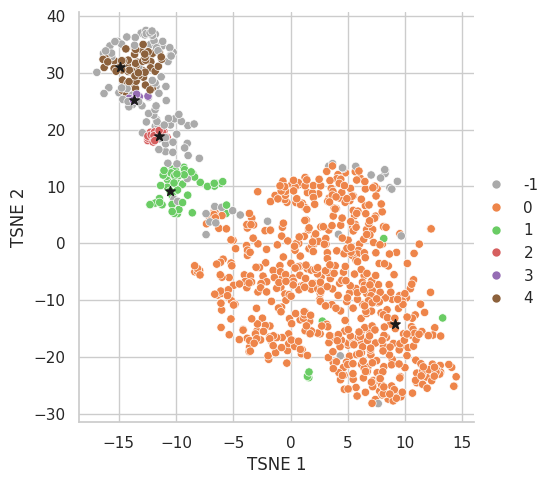
\includegraphics[width=\textwidth]{../results/images/tsclust_density_tsne.png}
        \caption{DBSCAN clustering tSNE.}
    \end{subfigure}
    \caption{Clusters and cluster medoids for hierarchical clustering and DBSCAN visualized with two dimensionality reduction techniques.}\label{fig:clusters}
\end{figure*}

We also visualized the clusters using tSNE on the DTW distance matrix.
We choose this projection for its ability of preserving the local structure of the dataset.
While tSNE was able to convey some information on the numeric relative dimensions of different clusters, and was able to visualize clusters nicely, in the end it proved less interesting, because of its inability of revealing the global structure of the dataset and of conveying the variable density of our clusters.

Inspection of the PCA visualization convinced us that extraction of clusters with a density-based method was viable.
Since a series of run with different radii failed to return any interesting clusters, we decided to pursue a different approach: we run OPTICS (with \texttt{minPts=4}) to completion on a reduced version of the dataset, using the first 5 components created by PCA (which capture more than 80\% of variance). We then visualized the reachability plot and choose an appropriate radius with which to run DBSCAN using the reachability distances computed by OPTICS.
DBSCAN detected 116 noise points and returned five clusters of varying sizes (C0: 594, C1:57, C2: 16, C3: 5 and C4: 62, see Fig. \ref{fig:tsclust_density_series}).

We computed the silhouette score for non noise points on the DTW distance matrix, in order to have results comparable with the other clustering methods.
We found that, while globally the silhouette was a little worse than for the previous methods (0.69), essentially no record showed signs of being misclassified.

Inspection of the PCA visualization (Fig. \ref{fig:density_pca}) shows that this method doesn't fall into the pitfalls of the hierarchical clustering, for example finding a good separation between C0 and C1.

However, while C0 and C1 are fully satisfactory, respectively clustering together instant hits and movies with a similar pattern to instant hits, but with a less explosive first weekend, it looks to us that the clustering of records with lower values on the first PCA component is more contentious because of DBSCAN's inability to detect clusters of different densities.
Arguably the `late bloomers' from C3 and C4 should be clustered together (probably with some noise points).
C2, despite its size, captured our interest, because it was able to detect a pattern no other clustering method was able to capture. It seems to us that movies in this cluster have a slow start at the box office, but, differently from our `late bloomers', they explode on the first weekend after the release and then display a behavior very similar to instant hits.
We hypothesized that this cluster was grouping together movies that were pre-released in a limited fashion.

\subsubsection{Distribution of shape-based clusters w.r.t. exogenous features}
\begin{figure}
    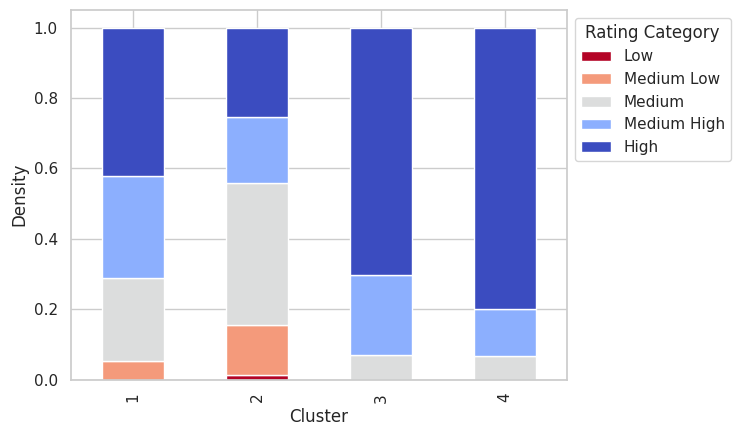
\includegraphics[width=\columnwidth]{../results/images/dist_clust_rating_cat.png}
    \caption{Distribution of binned rating by cluster (hierarchical).}
\end{figure}

In this analysis we concentrated our attention on instant hits from C3 and `late bloomers' from C2 returned by the hierarchical clustering.
We noticed that `late bloomers' have on average a lower average box office (median in the 100k) than instant hits (median in the millions).
This is a valuable finding, since we applied amplitude scaling on the time series before analysis.

In addition to that, we found that `late bloomers' are treated more favorably in terms of rating, as can be seen from  and receive on average more awards and nominations.
Action movies are severely underrepresented among `late bloomers' (only 5\% vs 38\% of records from C2 and 32\% globally), while dramatic movies are overrepresented, since, despite making up about half of the dataset, they make up more than 85\% of C3.

\subsubsection{Global structural features clustering}\label{sec:tsclust_features}
We ran hierarchical clustering on time series structural features experimenting with different linkage criteria and selecting the one that gave use the best dendrogram (Ward).
We obtained four clusters and a mean silhouette of 0.21 (it should be noted that we do not invite comparison with the silhouette obtained by shape-based methods, since this clustering was performed on an entirely different distance matrix).

From Fig. \ref{fig:tsclust_structure.png} we can see that also this clustering method was able to detect the patterns observed previously, albeit in a less marked way. C1 and C2 (which are later merged in a single cluster) are mainly made up of `late bloomers', while C3 and C4 group together instant hits (C3 and C4 are sisters).

\begin{figure}
    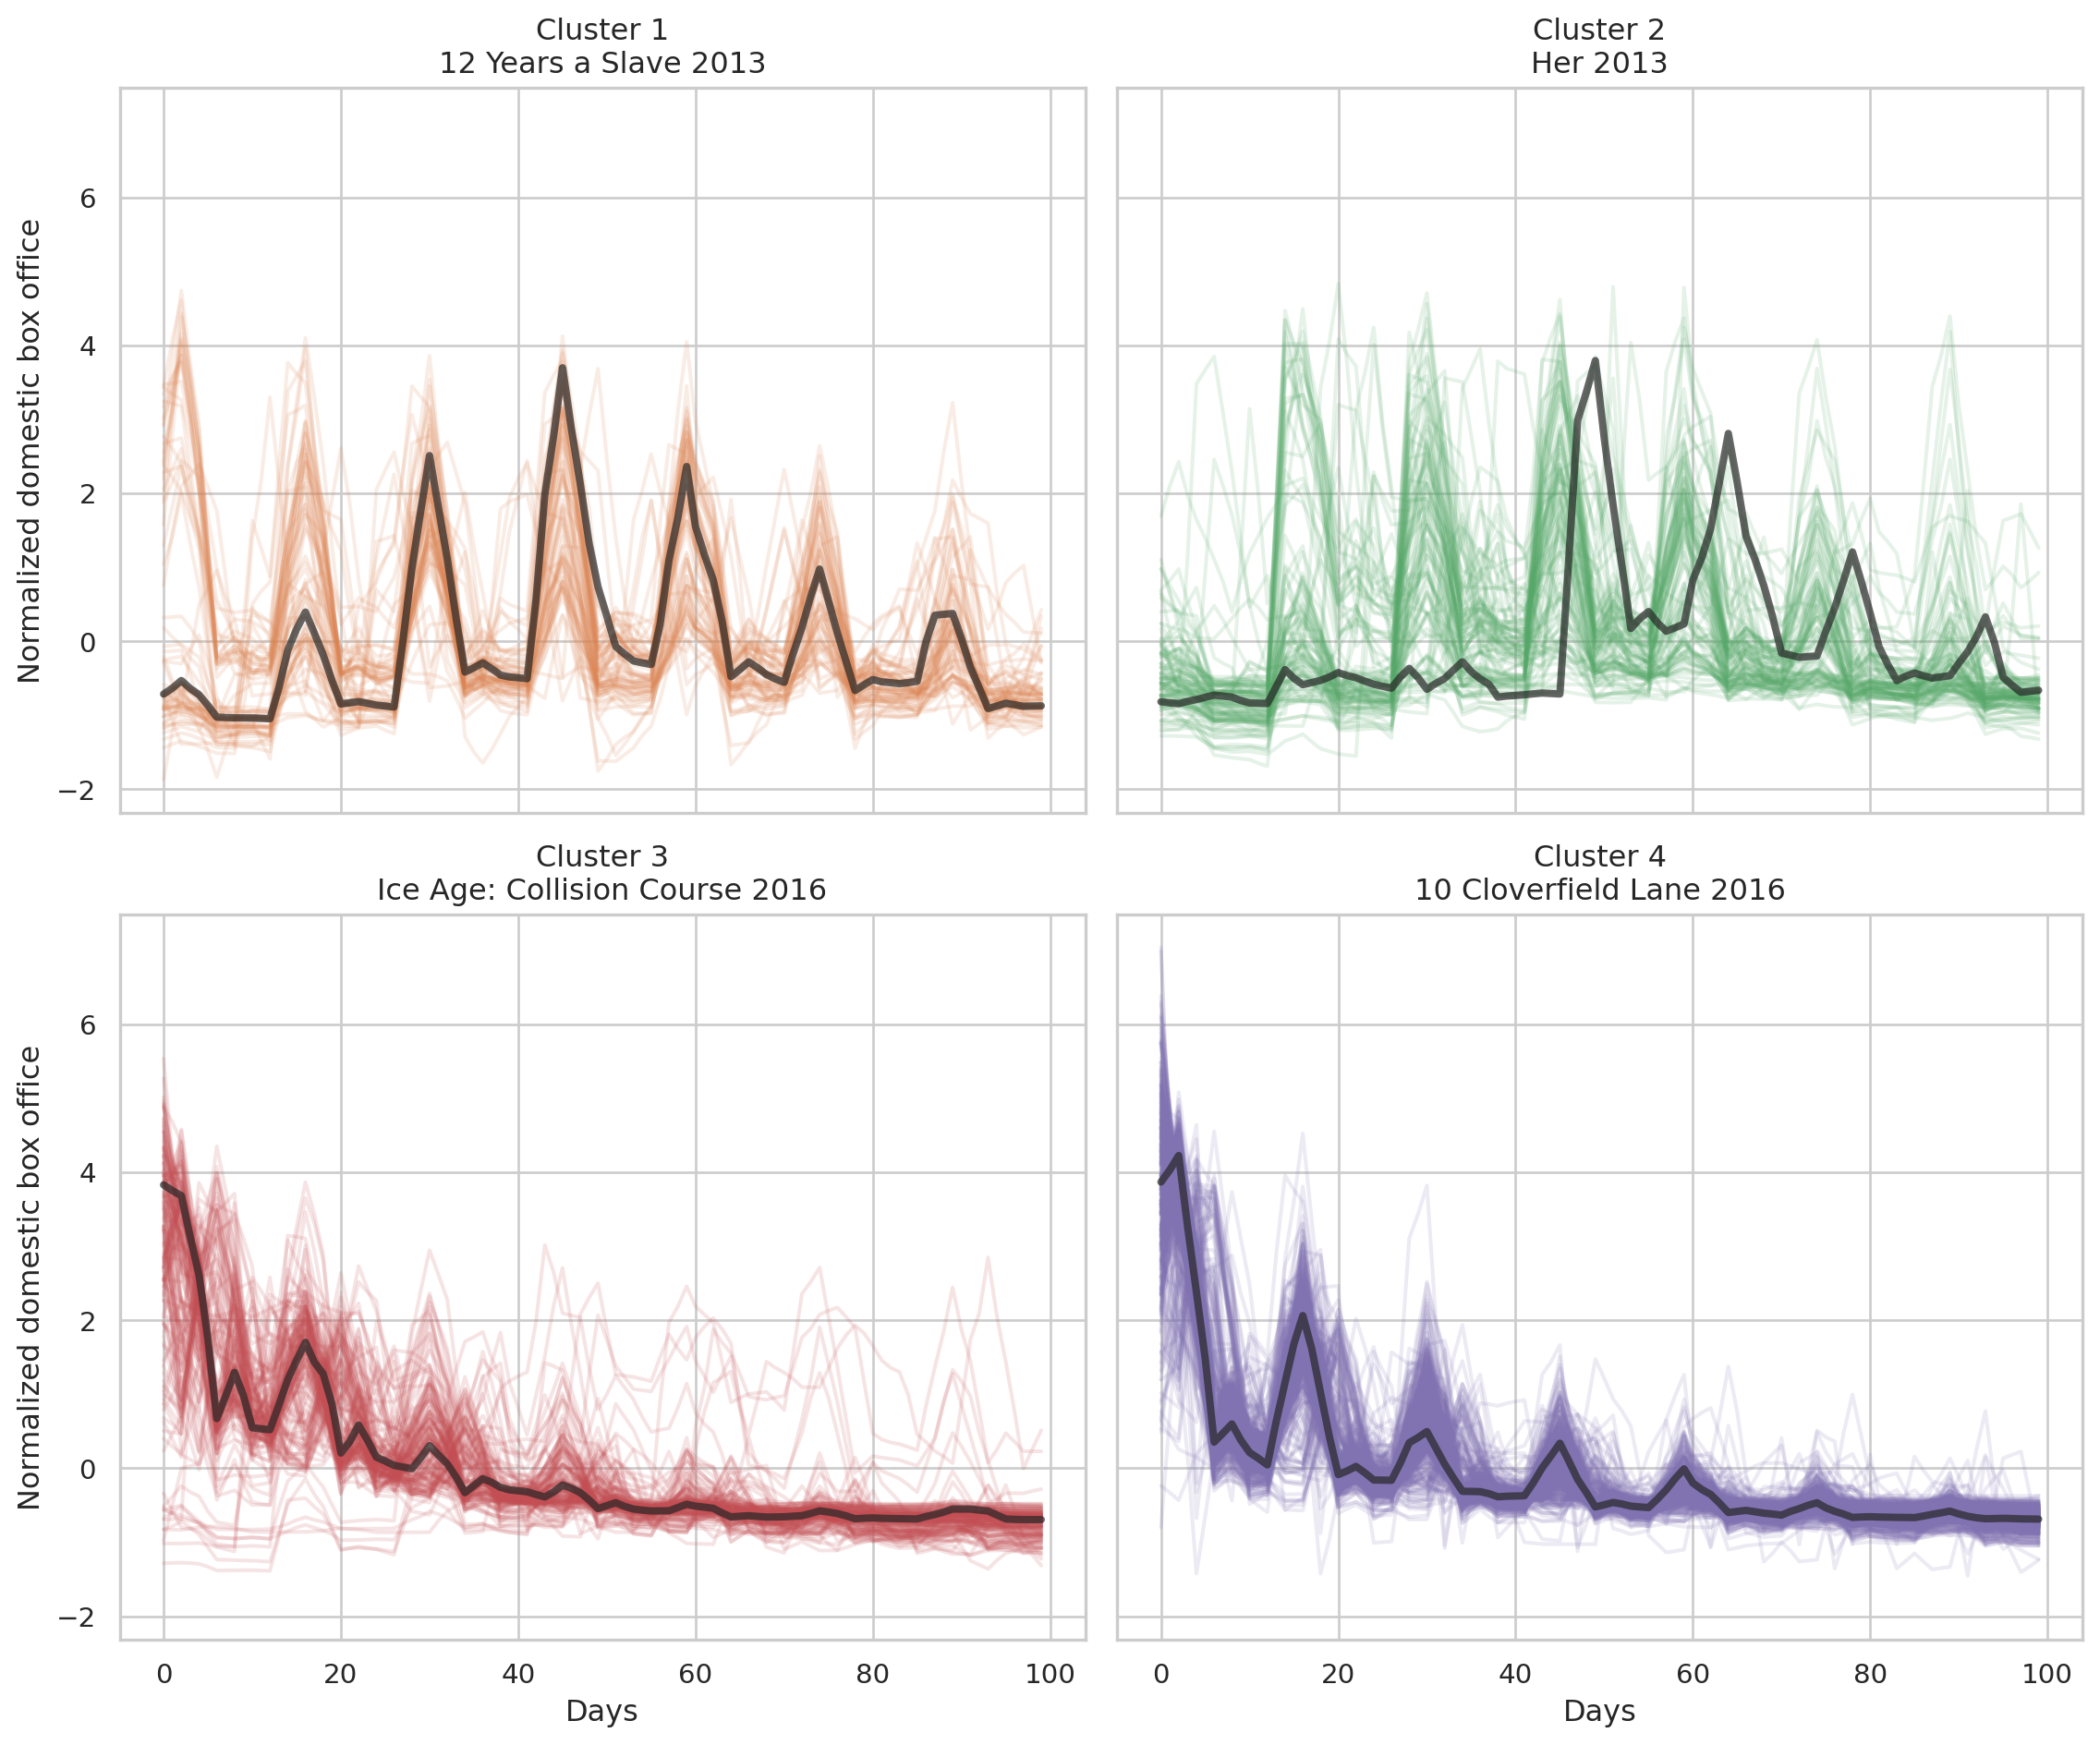
\includegraphics[width=\columnwidth]{../results/images/tsclust_structure.png}
    \caption{Clusters obtained by hierarchical clustering on structural features and respective cluster medoids (in black).}\label{fig:tsclust_structure.png}
\end{figure}

Analysis of clusters w.r.t. exogenous features showed very similar patters to those already observed in terms of rating, binned rating, awards, nominations, distribution of action and dramatic movies.